\documentclass[tikz,border=5pt]{standalone}
\usepackage{amsmath}
\usetikzlibrary{positioning,arrows.meta}

\begin{document}
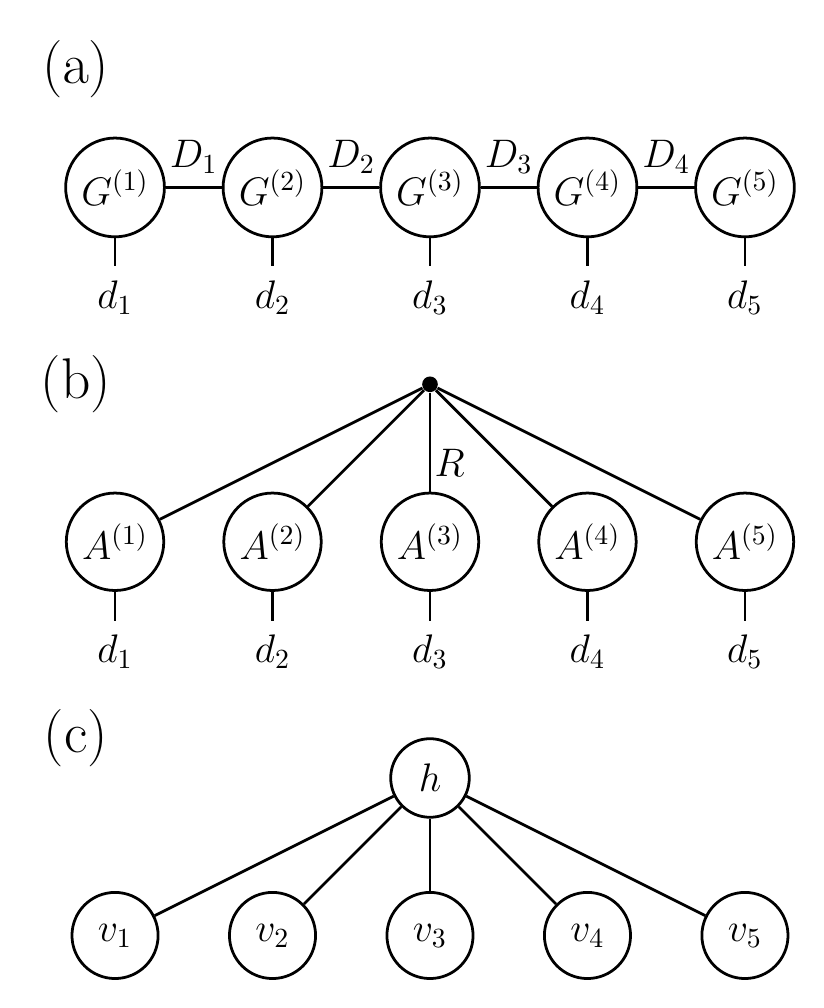
\begin{tikzpicture}[
  node/.style={circle,draw,inner sep=3pt,line width=1pt},
%  arr/.style={line width=1pt},
%  arr/.style={-{Stealth}},
  level distance=1.2cm,
  sibling distance=1.6cm
]

\Large

% (a)
\node at (-4.5,0.5) {\huge{(a)}};
\node[node] (G1) at (-4,-1) {$G^{(1)}$};
\node[node] (G2) at (-2,-1) {$G^{(2)}$};
\node[node] (G3) at (0,-1) {$G^{(3)}$};
\node[node] (G4) at (2,-1) {$G^{(4)}$};
\node[node] (G5) at (4,-1) {$G^{(5)}$};

\foreach \i/\j in {1/2,2/3,3/4,4/5}
  \draw[line width=1pt] (G\i) -- node[above]{$D_{\i}$} (G\j);

\foreach \i in {1,2,3,4,5}
  \draw[line width=1pt] (G\i) -- ++(0,-1) node[below]{$d_{\i}$};

% (b)
\node at (-4.5,-3.5) {\huge{(b)}};
\node[fill, circle, inner sep=2pt] (rootB) at (0,-3.5) {};
\node[node] (A1) at (-4,-5.5) {$A^{(1)}$};
\node[node] (A2) at (-2,-5.5) {$A^{(2)}$};
\node[node] (A3) at (0,-5.5)  {$A^{(3)}$};
\node[node] (A4) at (2,-5.5)  {$A^{(4)}$};
\node[node] (A5) at (4,-5.5)  {$A^{(5)}$};

\foreach \i in {1,2,3,4,5}
%  \draw[line width=1pt] (rootB) -- node[right]{$R$} (A\i);
  \draw[line width=1pt] (rootB) -- node[]{} (A\i);
\node[] at (0.25,-4.5) {$R$};

\foreach \i in {1,2,3,4,5}
  \draw[line width=1pt] (A\i) -- ++(0,-1) node[below]{$d_{\i}$};

% (c)
\node at (-4.5,-8) {\huge{(c)}};
\node[node] (rootC) at (0,-8.5) {$~h~$};
\node[node] (v1) at (-4,-10.5) {$~v_{1}~$};
\node[node] (v2) at (-2,-10.5) {$~v_{2}~$};
\node[node] (v3) at (0,-10.5)  {$~v_{3}~$};
\node[node] (v4) at (2,-10.5)  {$~v_{4}~$};
\node[node] (v5) at (4,-10.5)  {$~v_{5}~$};

\foreach \i in {1,2,3,4,5}
  \draw[line width=1pt] (rootC) -- (v\i);

\end{tikzpicture}
\end{document}

